\documentclass[conference]{IEEEtran}
\IEEEoverridecommandlockouts
% The preceding line is only needed to identify funding in the first footnote. If that is unneeded, please comment it out.
%Template version as of 6/27/2024

\usepackage{cite}
\usepackage{amsmath,amssymb,amsfonts}
\usepackage{algorithmic}
\usepackage{graphicx}
\usepackage{textcomp}
\usepackage{xcolor}
\usepackage{bm}
\ifCLASSOPTIONcompsoc
\usepackage[caption=false,font=normalsize,labelfon
t=sf,textfont=sf]{subfig}
\else
\usepackage[caption=false,font=footnotesize]{subfi
g}
\fi

\def\BibTeX{{\rm B\kern-.05em{\sc i\kern-.025em b}\kern-.08em
    T\kern-.1667em\lower.7ex\hbox{E}\kern-.125emX}}


\begin{document}

\title{Semantic Image Generation and Transmission (SIGT) for Optimized Wireless Communication\\

\thanks{This work was supported by Tsinghua University Student Research Training program, All authors are with the Center for Aerospace Information Network Research.}
}



\maketitle

\begin{abstract}
    Semantic communication optimizes the trade-off between computing power and transmission rate, potentially extending beyond Shannon capacity. We propose the Semantic Image Generation Transmission (SIGT) technique, which reduces communication latency, surpasses rate constraints, and preserves key information integrity. Experimental results show that SIGT outperforms conventional image generation methods in LPIPS and FID, demonstrating its superior efficiency for multimodal semantic communication.
\end{abstract}

\begin{IEEEkeywords}
Semantic Communication,AIGC,Wireless Communication
\end{IEEEkeywords}

\section{Introduction}
As communication bandwidth becomes increasingly scarce and computational demands grow, future wireless communication paradigms must address rising expectations for higher transmission rates, reliability, and efficiency. Traditional communication methods have approached the Shannon limit, making it challenging to meet these demands with existing technologies.
Recent developments in generative AI have opened up possibilities for new communication paradigms. Using generative AI to empower semantic communication is an effective way to fulfill these requirements\cite{10639525,kalita2024largelanguagemodelsllms}, and several studies have applied this idea to 3D SC and image reconstruction.\cite{jiang2024largegenerativemodelassisted,jiang2024visuallanguagemodelbased}

This paper introduces the SIGT system for image transmission. The original image is segmented into critical and non-critical parts. The critical part is transmitted using traditional coding to minimize distortion, while non-critical parts are conveyed through AI to generated textual descriptions. This multimodal approach achieves significant compression while ensuring the integrity of key information.


\section{Proposed SIGT Framework}

\subsection{Overview}
The SIGT system (Fig.~\ref{Fig.1}) processes an image $\bm{X}$ by dividing it into:
\begin{itemize}
    \item \textbf{Critical Region} ($\bm{Y}_I$): Key objects or important parts of the scene.
    \item \textbf{Non-Critical Region} (described by $\bm{Y}_T$): Background or less informative areas, represented as textual prompts.
\end{itemize}

By transmitting critical portions as image data and encoding non-critical portions as text, the receiver uses generative models to inpaint and reconstruct the full image. The result is a semantic communication strategy that can achieve substantial bandwidth savings without compromising essential information.

\begin{figure}[htbp]
    \centerline{\includegraphics[width=9cm]{1.png}}
    \caption{Communication flow of the proposed SIGT system.}
    \label{Fig.1}
\end{figure}

\subsection{Data and Mathematical Characterization of the Transmission Stream}

Let $\bm{X}$ be an image drawn from a distribution $\mathcal{X}$, where $\mathcal{X}$ denotes the probability space of possible source images. Formally, $\mathcal{X}$ is a distribution on $\mathbb{R}^{H\times W \times C}$ characterizing the probability of encountering any image. The segmentation model $S(\cdot)$ extracts critical regions:
\begin{align}
\bm{Y}_I = S(\bm{X}),
\end{align}
where $S: \mathbb{R}^{H \times W \times C} \to \mathbb{R}^{D_I}$ and $D_I < HWC$.

A description model $D(\cdot)$ outputs a textual sequence that semantically describes the non-critical parts of the image:
\begin{align}
\bm{Y}_T = D(\bm{X}),
\end{align}
where $D: \mathbb{R}^{H\times W \times C} \to \mathcal{T}^{L}$, and $\mathcal{T}^{L}$ denotes the space of textual sequences of length $L$. This space $\mathcal{T}^{L}$ can be understood as an $L$-dimensional token embedding space, where each token is represented in a high-dimensional vector space (e.g., word embeddings or subword embeddings) and $L$ reflects the length of the textual description.

We form a joint representation:
\begin{align}
\bm{Y} = (\bm{Y}_I,\bm{Y}_T).
\end{align}

A semantic source encoder $\mathcal{F}_{\theta}$ compresses $\bm{Y}$ into a low-dimensional latent vector $\bm{Y'}$:
\begin{align}
\bm{Y'} = \mathcal{F}_{\theta}(\bm{Y}) = E_{\theta I}(\bm{Y}_I) + E_{\theta T}(\bm{Y}_T) + \epsilon,
\end{align}
where $E_{\theta I}$ and $E_{\theta T}$ are encoders for image and text components, respectively, and $\epsilon$ represents residual encoding noise.

The channel encoder $\mathcal{H}_{\alpha}$ maps $\bm{Y'}$ into a codeword $\bm{Z}$ for transmission:
\begin{align}
\bm{Z} = \mathcal{H}_{\alpha}(\bm{Y'}).
\end{align}
The noisy channel introduces additive white Gaussian noise (AWGN):
\begin{align}
\bm{Z'} = \bm{Z} + \eta, \quad \eta\sim \mathcal{N}(0,\sigma_{\eta}^2 I).
\end{align}

At the receiver, the channel decoder $\mathcal{H}_{\beta}$ attempts to recover:
\begin{align}
\bm{\hat{Y}'} = \mathcal{H}_{\beta}(\bm{Z'}).
\end{align}

The semantic destination decoder $\mathcal{F}_{\phi}$ reconstructs:
\begin{align}
(\hat{\bm{Y}}_I,\hat{\bm{Y}}_T) = \mathcal{F}_{\phi}(\bm{\hat{Y}'}).
\end{align}

Given $\hat{\bm{Y}}_I$ and the textual prompt $\hat{\bm{Y}}_T$, the inpainting model $I(\cdot)$ reconstructs the full image:
\begin{align}
\hat{\bm{X}} = I(\hat{\bm{Y}}_I,\hat{\bm{Y}}_T).
\end{align}

A suitable distortion measure ensures semantic fidelity:
\begin{align}
d(\bm{X},\hat{\bm{X}}) &= \lambda_I \|S(\bm{X}) - \hat{\bm{Y}}_I\|_2^2 \nonumber \\ 
 &+\lambda_T D_{\text{NLP}}(D(\bm{X}),\hat{\bm{Y}}_T) + \lambda_{vis}\|\bm{X}-\hat{\bm{X}}\|_2^2,
\end{align}
where $D_{\text{NLP}}(\cdot,\cdot)$ is a semantic similarity measure in text space, and $\lambda_I,\lambda_T,\lambda_{vis}$ weight the contributions of critical region accuracy, textual fidelity, and overall visual similarity.

This construction highlights how SIGT departs from traditional bit-based models to focus on transmitting semantic content. By leveraging $\mathcal{X}$ (the distribution of images) and $\mathcal{T}^{L}$ (the textual embedding space), SIGT ensures that even when data is compressed and partially represented as text, essential meaning is preserved.

\subsection{Insight}\label{Baseline choose}

The key insight of SIGT is that not all parts of an image are equally important. Traditional approaches strive to transmit all pixels with equal fidelity, pushing against bandwidth and rate constraints. By identifying a small, critical subset of image features that must be preserved and representing the rest as a textual prompt, we reduce the data load dramatically. Generative AI models at the receiver then reconstruct the full image using these essential elements as guidance, effectively operating beyond classical rate-distortion limits. The textual prompt stabilizes the generative process, reducing randomness and helping achieve high semantic fidelity.

Crucially, we consider four strategies:
\begin{enumerate}
    \item \textbf{DirectlyGe}: Direct image generation from prompt only.
    \item \textbf{AllEdge}: Image generation using prompt and complete outlines.
    \item \textbf{HumanOnly}: Generation from critical human parts alone.
    \item \textbf{SIGT}: Generation from critical parts and semantic prompt, our proposed framework.
\end{enumerate}

Among these, SIGT outperforms its counterparts by optimally balancing the critical details transmitted as image data with semantic guidance through text, resulting in better alignment, fidelity, and visual quality.


To visualize the comparative performance, Fig.\ref{combined} illustrates the relationship between the sliding average of the reconstructed area share (which correlates with the compression ratio) and the LPIPS score. As observed, when no prompt is provided in the model input, the LPIPS curve follows a pattern akin to geometric Brownian motion.


\begin{figure}[htbp]
    \centering
    \fbox{
    \begin{minipage}{1\columnwidth} % 设置 fbox 宽度与列宽一致
        \begin{minipage}{0.4\textwidth}
            % A: 图像
            
            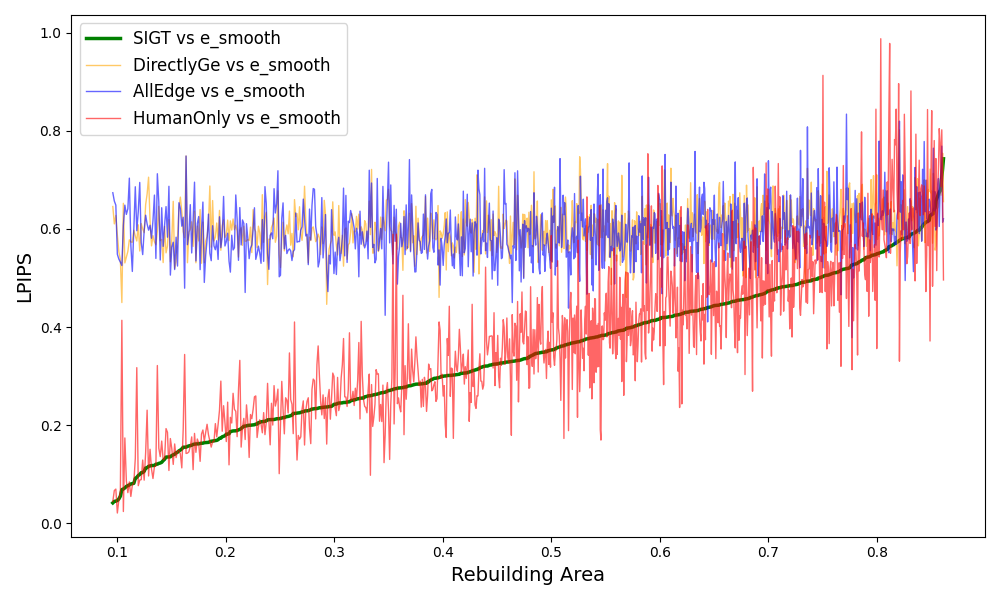
\includegraphics[width=1.15\columnwidth]{LPIPS.png}
            \label{LPIPS}
        \end{minipage}%
        \begin{minipage}{0.25\textwidth}
            % B: 公式部分
            \fontsize{7}{8}\selectfont
            \[
                \quad\quad dD_{\bar{s}} = \mu D_{\bar{s}} \, d\bar{S} + (\sigma - \xi) D_{\bar{s}} \, dW(\bar{S})
            \]
            \[
                \quad\quad d \ln(D_{\bar{s}}) = \mu \, d\bar{S} + (\sigma - \xi) \, dW(\bar{S})
            \]
            \[
                \quad\quad E[\ln(D_{\bar{s}})] = \ln(D_0) + \mu \bar{S} - \frac{1}{2} (\sigma - \xi)^2 \bar{S}
            \]
        \end{minipage}%
        \\ % 强制换行
        \begin{minipage}{\textwidth}
            % C: 参数说明部分
            \textbf{In this formulation:}
            \begin{itemize}
                \item \( \mu \): The model's inpainting ability based on the image.
                \item \( \sigma \): Intrinsic randomness without the prompt.
                \item \( \xi \): Reduction of randomness due to the prompt.
                \item \( \bar{S} \): Moving average of areas to be reconstructed.
                \item \( \mu Dd\bar{S} \) represents the deterministic trend, showing how the perceptual loss changes with the increasing reconstruction area \( \bar{S} \).

                \item\( \sigma DdW(\bar{S}) \) models the volatility, indicating randomness in the inpainting process.
                
                \item\( \xi DdW(\bar{S}) \) represents the correction due to the prompt, reducing the randomness.
            \end{itemize}
        \end{minipage}
    \end{minipage}
    }
    \caption{Mathmatical model for LPIPS}
    \label{combined}
\end{figure}

This equation effectively models the perceptual loss during image reconstruction, accounting for both deterministic trends and random noise, and provides a framework for managing the challenges of image generation, inpainting, and restoration.


We model the perceptual loss during image reconstruction using the following equation:

\[
    dD_{\bar{s}} = \mu D_{\bar{s}} \, d\bar{S} + \sigma D_{\bar{s}} \, dW(\bar{S}) - \xi D_{\bar{s}} \, dW(\bar{S})
    \]
    This can be rewritten as:
    \[
    dD_{\bar{s}} = \mu D_{\bar{s}} \, d\bar{S} + (\sigma - \xi) D_{\bar{s}} \, dW(\bar{S})
    \]
    Where \( \mu \) is the deterministic trend term, \( \sigma \) is the randomness (volatility), \( \xi \) is the coefficient that represents the reduction of randomness introduced by the prompt, and \( dW(\bar{S}) \) is the increment of the standard Brownian motion.

    To derive \( \ln(D_{\bar{s}}) \), we first take the logarithm of \( D_{\bar{s}} \). Using the logarithmic differential rule, we get:
    \[
    d \ln(D_{\bar{s}}) = \frac{1}{D_{\bar{s}}} \, dD_{\bar{s}}
    \]
    Substituting the differential equation from earlier:
    \[
    d \ln(D_{\bar{s}}) = \frac{1}{D_{\bar{s}}} \left( \mu D_{\bar{s}} \, d\bar{S} + (\sigma - \xi) D_{\bar{s}} \, dW(\bar{S}) \right)
    \]
    Simplifying, we get:
    \[
    d \ln(D_{\bar{s}}) = \mu \, d\bar{S} + (\sigma - \xi) \, dW(\bar{S})
    \]

    By Itô's Lemma, for the logarithmic function \( f(D_{\bar{s}}) = \ln(D_{\bar{s}}) \), we know:
    \[
    d \ln(D_{\bar{s}}) = \frac{dD_{\bar{s}}}{D_{\bar{s}}} - \frac{1}{2} \left( \frac{d^2 D_{\bar{s}}}{D_{\bar{s}}^2} \right)
    \]
    Since \( d^2 D_{\bar{s}} \) is related to \( d\bar{S} \) and \( dW(\bar{S}) \), and ignoring the second-order terms, we arrive at:
    \[
    d \ln(D_{\bar{s}}) = \mu \, d\bar{S} + (\sigma - \xi) \, dW(\bar{S})
    \]

    To derive the expectation, we integrate the equation above. We have:
    \[
    \ln(D_{\bar{s}}) = \ln(D_0) + \int_0^{\bar{S}} \mu \, d\bar{S} + \int_0^{\bar{S}} (\sigma - \xi) \, dW(\bar{S})
    \]
    The first integral is the deterministic part, and the second integral is the stochastic part. The expectation of the stochastic part is 0, because the expectation of the standard Brownian motion is 0. Thus, we get:
    \[
    E[\ln(D_{\bar{s}})] = \ln(D_0) + \mu \bar{S} - \frac{1}{2} (\sigma - \xi)^2 \bar{S}
    \]




\subsection{Model Selection}
To optimize the quality and stability of the reconstructed images, we propose that the source side provides a detailed description to mitigate the randomness caused by the absence of a prompt. Additionally, when a critical component of the image is missing, the generation effect is fundamentally similar to that of the direct prompt generation, thus providing only the key part of the image offers a meaningful initial condition for reconstruction.

For this purpose, we deploy a Semantic Attention Mechanism (SAM) model at the source side to accurately identify and extract the critical regions \( H \) and mask \( M \) from the image. A picture captioning model is used to generate the descriptive text \( P \), which provides a semantic context for the image. At the receiver side, the picture reconstruction model is employed to regenerate the final image.

To reduce computational complexity and improve processing efficiency, we modularize the tasks by selecting specialized generative AI models that perform exceptionally well in single-task processing and exhibit lower computational demand. These models unlock the performance advantages of our system without imposing excessive computational burdens.

Furthermore, when generating images based on SAM-segmented images, the generalization capabilities of graphical text models come into play. The generated content based on the text description \( P \) is placed in a more semantically meaningful position by the model. However, the contours and labels provided by SAM may introduce extraneous information that could negatively impact the accuracy of the graphical text model, potentially degrading the quality of the generated images. Therefore, the only critical requirement for the SAM model is that it accurately segments the important parts of the image, while the non-critical areas can be reconstructed from the semantic description.

To this end, we select the Monkey model \cite{li2023monkey} for image description generation, as it has demonstrated strong performance in generating high-quality captions for images. For semantic segmentation, we choose ResNet50 \cite{he2016deep}, which is widely known for its robustness and efficiency in segmentation tasks. Finally, Stable Diffusion Inpainting \cite{Rombach_2022_CVPR} is employed for image reconstruction at the host side, as it has shown exceptional capability in handling inpainting tasks, significantly improving semantic consistency after multiple iterations, which aligns with the requirements of our system.

These models were specifically chosen for their ability to perform well on individual tasks while maintaining a low computational cost. This combination of models ensures that the system can deliver high-quality image transmission and reconstruction with efficient use of computational resources, making it suitable for real-time deployment in wireless communication systems.




\section{Simulation Result}

\begin{figure}[!t]
    \centering
    {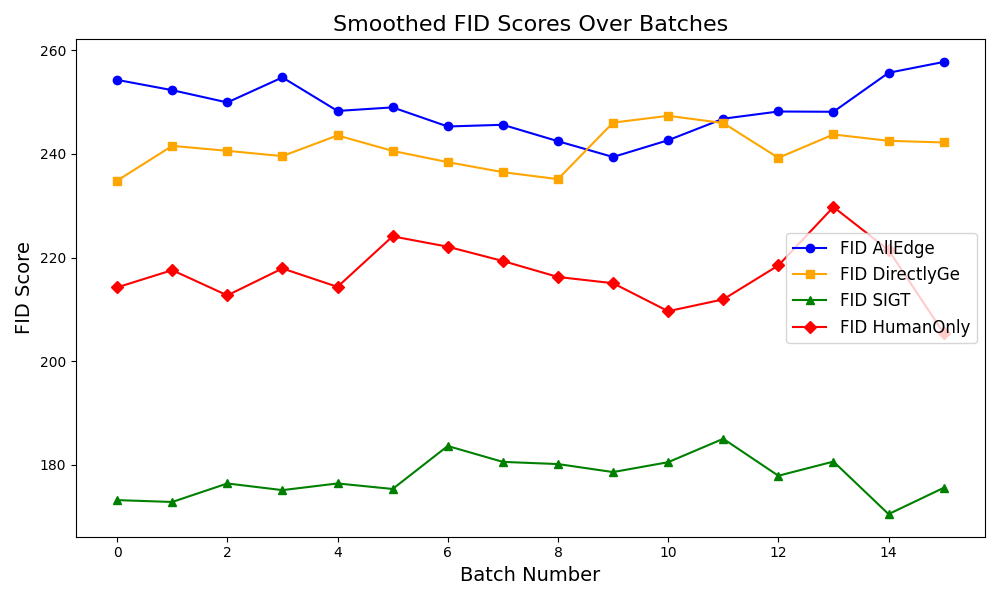
\includegraphics[width=0.9\columnwidth]{FID.png}}
    \caption{FID Distributions and Performance Improvement (Mean-based)}
    \label{FID}
\end{figure}

To comprehensively assess the performance of the Semantic Image Generation Transmission (SIGT) technique, we evaluate it using two key metrics: LPIPS and  FID. These metrics are crucial for assessing different aspects of image quality and consistency, including perceptual quality, semantic integrity, and spatial accuracy.

\begin{itemize}
    \item \textbf{LPIPS (Learned Perceptual Image Patch Similarity)}: This metric quantifies perceptual similarity between generated and reference images. A lower LPIPS score indicates that the generated image closely resembles the original in terms of human visual perception.
    \item \textbf{FID (Fréchet Inception Distance)}: FID measures the distance between the distributions of real and generated images in a feature space, capturing both the quality and diversity of the generated images. A lower FID indicates better quality and diversity.
    
\end{itemize}

We conducted a systematic simulation experiment on a dataset of 900 randomly selected photographs from the PIPA dataset. These images were processed using SIGT and a baseline image generation method. The baseline was chosen is attentioned above in \ref{Baseline choose}.

The results of the simulations are presented in Fig.\ref{LPIPS}and Fig.\ref{FID} for both SIGT and the baseline method. The numerical results indicate that SIGT significantly outperforms the baseline in  metrics. Specifically, SIGT achieves a 42\% improvement in LPIPS, more than 33\% improvement in FID, compared to the baseline. These improvements underscore the effectiveness of the SIGT framework in generating high-quality images that are perceptually and structurally closer to the original inputs.


The reduction in LPIPS and FID underscores SIGT's ability to produce perceptually pleasing images that are also statistically consistent with the original image distribution. By cleverly combining partial image data (critical parts) with powerful generative models guided by semantic prompts, SIGT delivers reconstructed images that look not only similar but also naturally coherent.

Since SIGT relies on textual prompts, the length $L$ of the textual sequence and the complexity of $\mathcal{T}^{L}$ are key factors. In practice, $L$ is chosen to provide sufficient semantic detail without overwhelming the receiver. This trade-off ensures that SIGT remains scalable to higher resolutions and more complex scenes while maintaining reduced bandwidth usage.

These results validate the competitive performance of SIGT, demonstrating its potential as an advanced image transmission method that excels in both quality and efficiency. The improvements across all three metrics highlight SIGT's ability to outperform conventional methods, offering a promising solution for high-quality image generation and transmission in future communication systems. These findings suggest that SIGT could be a key enabler for efficient and reliable wireless transmission, particularly in applications where both perceptual quality and semantic content preservation are crucial.



\section{Conclusion}
This paper introduced SIGT, a novel semantic communication framework that leverages generative AI models to reduce transmission costs while preserving essential information. By decomposing the image into critical and non-critical parts, and using textual prompts to guide generative reconstruction, SIGT surpasses conventional limits in perceptual quality and semantic fidelity.

Our experiments confirm that SIGT outperforms traditional approaches in LPIPS and FID metrics, affirming its promise in delivering both high semantic integrity and bandwidth efficiency. SIGT exemplifies how semantic communication can transcend classical constraints, heralding new opportunities for rich and meaningful information transfer in future wireless networks.

\begin{thebibliography}{1}

\bibitem{10639525}
Z.~Qin, L.~Liang, Z.~Wang, S.~Jin, X.~Tao, W.~Tong, and G.~Y. Li, ``Ai empowered wireless communications: From bits to semantics,'' \emph{Proceedings of the IEEE}, vol. 112, no.~7, pp. 621--652, 2024.

\bibitem{kalita2024largelanguagemodelsllms}
A.~Kalita, ``Large language models (llms) for semantic communication in edge-based iot networks,'' 2024. [Online]. Available: https://arxiv.org/abs/2407.20970


\bibitem{jiang2024largegenerativemodelassisted}
F.~Jiang, Y.~Peng, L.~Dong, K.~Wang, K.~Yang, C.~Pan, and X.~You, ``Large generative model assisted 3d semantic communication,'' 2024. [Online]. Available: https://arxiv.org/abs/2403.05783


\bibitem{jiang2024visuallanguagemodelbased}

F.~Jiang, C.~Tang, L.~Dong, K.~Wang, K.~Yang, and C.~Pan, ``Visual language model based cross-modal semantic communication systems,'' 2024. [Online]. Available:https://arxiv.org/abs/2407.00020


\bibitem{li2023monkey}
Z.~Li, B.~Yang, Q.~Liu, Z.~Ma, S.~Zhang, J.~Yang, Y.~Sun, Y.~Liu, and X.~Bai, ``Monkey: Image resolution and text label are important things for large multi-modal models,'' \emph{arXiv preprint arXiv:2311.06607}, 2023.



\bibitem{he2016deep}
K.~He, X.~Zhang, S.~Ren, and J.~Sun, ``Deep residual learning for image recognition,'' in \emph{Proceedings of the IEEE conference on computer vision and pattern recognition}, 2016, pp. 770--778.

\bibitem{Rombach_2022_CVPR}
R.~Rombach, A.~Blattmann, D.~Lorenz, P.~Esser, and B.~Ommer, ``High-resolution image synthesis with latent diffusion models,'' in \emph{Proceedings of the IEEE/CVF Conference on Computer Vision and Pattern Recognition (CVPR)}, June 2022, pp. 10\,684--10\,695.

\end{thebibliography}

\end{document}
